
\documentclass[10pt,a4paper]{article}
    \usepackage[utf8]{inputenc}
    \usepackage{xcolor}
    % \usepackage[utf8x]{inputenc} % para poder usar tildes en archivos UTF-8
    \usepackage[spanish,es-tabla]{babel}
    \usepackage{verbatim}
    \usepackage{clrscode3e}
    \usepackage{amssymb}
    \usepackage{amsmath}
    \usepackage{amsfonts} % for the \checkmark command 
    \usepackage{graphicx}
    \usepackage{float}
    \usepackage{pdfpages}
    \usepackage{enumerate}
    \usepackage{caption}
    \usepackage{subcaption}
    \usepackage[left=3cm, right=3cm, top=2cm]{geometry}
% \documentclass[10pt,a4paper]{article}
% \usepackage[utf8x]{inputenc} % para poder usar tildes en archivos UTF-8
% \usepackage[spanish,es-tabla]{babel}
% \usepackage{verbatim}
% \usepackage{amsmath}
% \usepackage{clrscode3e}
% \usepackage{amssymb}
% \usepackage{graphicx}
% \usepackage{float}
% \usepackage{pdfpages}

%\usepackage{bibtex}

%\usepackage{a4wide} % márgenes un poco más anchos que lo usual

\usepackage{caratula} % Se puede descargar en ~> https://github.com/bcardiff/dc-tex
\usepackage[breaklinks=true]{hyperref}


\begin{document} % Todo lo que escribamos a partir de aca va a aparecer en el documento.

%fran
%\sloppy

% Completar los datos de la caratula
\titulo{Trabajo Práctico 1 - Eligiendo justito} 
\fecha{\today}
\materia{Algoritmos y Estructuras Datos III}
\grupo{Grupo "Kubrak"}

% Completar los integrantes del grupo:)
\integrante{Cristian Kubrak}{456/15}{Kubrakcristian@gmail.com}

\maketitle

% \par \textbf{Abstract:} El objetivo de este trabajo es resolver el problema de la suma de
% subconjuntos mediante 3 diferentes t\'ecnicas: Fuerza Bruta, Backtracking y 
% Programaci\'on din\'amica para luego analizar cu\'al de ellas resulta mejor aplicar seg\'un el contexto.

\tableofcontents
% \par  \textbf{Palabras clave:} subset sum - brute force - Backtracking - Programaci\'on din\'amica
% Aca comienzan a escribir su informe


\newpage

\section{Introducción}
\par Dado un conjunto $S = \{v_1,v_2,...,v_n\}$, y un valor objetivo $V$, se busca decidir si existe un subconjunto
de items de $S$ que sumen exactactamente el valor objetivo $V$. En caso de existir dicho conjunto, se obtener la
m\'inima cardinalidad entre los subconjuntos que sumen $V$.

\par Para resolver este problema, se utilizaron tres t\'ecnicas diferentes: \emph{Fuerza Bruta}, \emph{BackTracking}
y \emph{Programaci\'on din\'amica}.

\subsubsection{Fuerza Bruta}
\par Para el caso de la fuerza bruta, se busca armar todos los posibles subconjuntos del conjunto $S$ para luego realizar
la suma y verificar si el n\'umero obtenido es $V$.

\subsubsection{BackTracking}
\par El BackTracking es un m\'etodo de fuerza bruta inteligente: en el peor caso se comporta como un m\'etodo de fuerza
bruta, pero no se investigan las posibilidades que por \emph{optimalidad } o \emph{factibilidad} se descartan.
Para descartar por \emph{optimalidad}, una vez hallada una soluci\'on se guarda el cardinal. A la hora de analizar nuevas
posibles soluciones, si el el cardinal del nuevo subconjunto excede el actual m\'inimo, es descartado. \par
Por otro lado, para descartar por \emph{factibilidad} a la hora de armar un subconjunto se lo arma elemento por elemento
y en caso de ya superar el valor $V$, se dejan de agregar elementos (ya que todos son no negativos).


\subsubsection{Programaci\'on din\'amica}
\par Para este enfoque, se plantea el problema a resolver como un problema recursivo a partir de subproblemas.
Al haber varios subproblemas superpuestos, se guarda su soluci\'on en un diccionario de r\'apido acceso. Al tener las 
soluciones al subproblema almacenadas, no se realiza m\'as de una vez la misma operaci\'on.

\subsection{Ejemplos del problema}
\subsubsection{Caso A}
Sea un conjunto $S = \{ 4, 10,3,1,1\}$ y $V=5$. Los posibles subconjuntos que suman 5 son: $\{4,1 \}$ y $\{3,1,1\}$
los cuales tienen cardinal 2 y 3 respectivamente. Dado que el inter\'es de este problema es encontrar la 
m\'inima cardinal para la cual existe un subconjunto tal que la suma de sus elementos es exactactamente $V$, la 
soluci\'on para este caso es $2$.
\subsubsection{Caso B}
Sea el conjunto $S = \{ 5, 7 ,3,2\}$ y $V=6$. No extiste ning\'un subconjunto tal que la suma de los elementos
sea exactactamente $6$, raz\'on por la soluci\'on a este problema es $-1$
\newpage

\section{Desarrollo}
\subsection{Fuerza Bruta}
Como primera opci\'on para resolver el problema se encuentra el algor\'itmo de Fuerza Bruta que, tal como el nombre
da a suponer, es una forma poco inteligente de buscar una soluci\'on ya que implica recorrer todo el \'arbol de 
soluciones:

\begin{codebox}
    \Procname{\proc{ResolverFuerzaBruta}(int V, int[] S, int i, int n) \textcolor{red}{O($2^n$)}}
    \li \If $i == -1$ \textcolor{red}{O($1$)}
        \Then
    \li        \If $V == 0$ : \textcolor{red}{O($1$)}
                \Then
    \li             \Return $0$ \textcolor{red}{O($1$)}
    \li         \Else: 
    \li                 \Return $n+1$\footnote{Si el algor\'itmo devulve un n\'umero mayor que $n$ significa que no existe soluci\'on} \textcolor{red}{O($1$)}
                \End
                \End

    \li \Return min(ResolverFuerzaBruta($V$,$S$,$i-1$,$n$), \\
   $\quad\quad\quad\quad\quad$ $1 +$ResolverFuerzaBruta($V-S[i]$,$S$,$i-1$,$n$)) \textcolor{red}{O($2^n$)}

    \end{codebox}


\begin{figure}[H] 
\centering
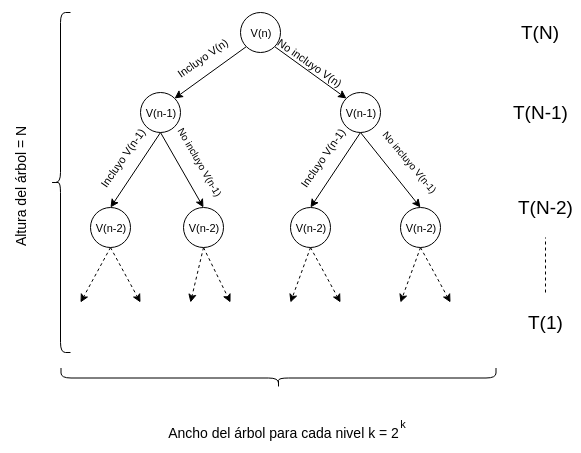
\includegraphics[width=.8\textwidth]{img/arbolRecurrencia.png}
\caption{\'Arbol de recurrencia}
\label{fig:arbolRecurrencia}
\end{figure}

Como la altura del \'arbol es de $n$ (el tama\~no del conjunto $S$) y el $\forall k, 1\leq k \leq n$ el ancho del
\'arbol para el nivel $k$ es de $2^k$, para recorrer todo el \'arbol se requieren:
\begin{equation}
    \sum_{i=0}^{n-1} 2^i*O(1) = \frac{2^{n}}{2-1} = 2^{n} \in O(2^n)
\end{equation}
Como se requieren $O(2^n)$ operaciones para investigar todas las soluciones y efectivamente se las investiga todas,
la complejidad del Fuerza Bruta es exactamente $O(2^n)$.

\subsection{Back Tracking}

\begin{codebox}
    \Procname{\proc{ResolverBackTracking}(int V, int[] S, int i, int n, int minParcial, int cardinalParcial) \textcolor{red}{O($2^n$)}} 
    % \li \If $i == -1$ \textcolor{red}{O($n*2^n$)}
    \li \If $cardinalParcial$ $>$ $minParcial$: \textcolor{red}{O($1$)}
        \Then
    \li        \Return $n+1$ \footnote{\label{bktrk}Si el algor\'itmo devulve un n\'umero mayor que $n$ significa que no existe soluci\'on} \End\textcolor{red}{O($1$)}
    \li \If $V == 0$: \textcolor{red}{O($1$)}
         \Then
    \li         $minParcial = cardinalParcial$ \textcolor{red}{O($1$)}
    \li         \Return $0$ \textcolor{red}{O($1$)}
    \End
    \li \If $i == -1$ \textcolor{red}{O($1$)}
        \Then
    \li                 \Return $n+1$ \textsuperscript{\ref{bktrk}} \textcolor{red}{O($1$)}
                \End
    \li \If $S[i]$ $>$ $V$: \textcolor{red}{O($1$)}
        \Then 
    \li         \Return  ResolverBackTracking($V$,$S$,$i-1$,$n$,$minParcial$,$cardinalParcial$)\textcolor{red}{O($2^n$)}
    \li    \Else:
    \li          \Return min(ResolverBackTracking($V$,$S$,$i-1$,$n$,$minParcial$,$cardinalParcial$),\textcolor{red}{O($2^n$)}
                            \\ $\qquad\qquad$$\qquad\quad\,\,$ $1+$ ResolverBackTracking($V-S[i]$,$S$,$i$,$n$,$minParcial$,$cardinalParcial+1$))



    \end{codebox}

\par Resulta f\'acil ver que la soluci\'on de Back Tracking es un caso especial del algor\'itmo de Fuerza Bruta,
salvo que gracias a las podas de \textit{optimalidad} y \textit{factibilidad} se evita investigar ciertas partes del
\'arbol de soluci\'on. A\'un as\'i, en el peor caso (por ejemplo un arreglo en el cual la suma de sus elementos no llega
a $V$) se termina comportando como Fuerza Bruta. Luego su complejidad resulta $O(2^n)$

\subsubsection{Poda por factibilidad}
\par La poda por \textit{factibilidad} se realiza en en la l\'inea 9 del pseudoc\'odigo. La misma consiste en
evaluar si el $S[i]$ es mayor estricto que el $V$. De as\'i serlo se excluye tal elemento en la soluci\'on ya que obviamente
har\'a que la suma de cualquier subconjunto que lo incluya exceder\'a el valor de $V$.


\subsubsection{Poda por optimalidad}
\par La poda por optimalidad se realiza en la l\'inea 1 del pseudoc\'odigo aunque las operaciones gracias a las
cuales funciona esta poda se realizan en las l\'ineas 4 y 12. En la primer l\'inea se evalua si el $cardinalParcial$
(el cardinal que lleva el subconjunto actual) es mayor estricto a $minParcial$ (el m\'inimo cardinal para el que
se encontr\'o un subconjunto cuya suma es exactamente $V$); de as\'i serlo, no tiene relevancia seguir evaluando
esa rama del \'arbol de soluciones ya que en caso de encontrar un subconjunto cuya suma sea $V$, su cardinal no ser\'a
el m\'inimo.
\par En la l\'inea 12, si se encontr\'o un subconjunto cuya suma sea $V$ (n\'otese que el $cardinalParcial$ debe
ser menor o igual al $minParcial$ gracias a la condici\'on en la l\'inea 1), $cardinalParcial$ pasa a ser el nuevo
$minParcial$ y se llega al caso base, por lo que se devuelve 0.
\par En la l\'inea 11 se busca el m\'inimo evaluan dos casos: incluir o no el elemento $S[i]$. N\'otese que en caso
de incluirlo el $cardinalParcial$ aumenta en 1.

\subsection{Programaci\'on Din\'amica}
\subsubsection{Correctitud}
Caracterizaci\'on de una solución \textbf{óptima} S para el problema original:
\par - Si $n \not\in$ $S$, entonces la mejor solución es $S =S_1$, siendo $S_1$ solución
óptima para \{$v_1 , v_2 , v_3 ,..., v_{n}$\} llegando al valor objetivo $V$
\par - Si $n \in S$, entonces la mejor solución es $S = \{n\} \cup S_2$, siendo $S_2$
solución óptima para \{$v_1 , v_2 , v_3 ,..., v_{n}$\} llegando al valor objetivo $V - v_n$
\par Por lo tanto, como esas son las únicas dos posibilidades, $S$ deberá ser la que use menos elementos entre 
$S_1$ y $\{n\} \cup S_2$
\par Usando esta caracterización, puedo elaborar una recursión
que calcule la cantidad óptima de elementos necesarios:
\begin{equation*}
  f(i,V)=\begin{cases}
    $\qquad\qquad$0 & \text{si $i=0$, $V=0$}.\\
    $\qquad\qquad$\infty & \text{si $i=0$, $V\neq 0$}.\\
    $\qquad\;\;\;$f($i$ $-$ $1$,$V$) & \text{si $i> 0$, $v_i > 0$}.\\
    min (f($i$ $-$ $1$,$V$),f($i$ $-$ $1$,$V$)) & \text{si $i> 0$, $v_i > 0$}.\\
  \end{cases}
\end{equation*}
\subsubsection{Principio de optimalidad}
\par Se puede ver que para este problema se puede aplicar el principio de optimalidad: una secuencia \'optima de
decisiones esta formada por subsecuencias que a su vez son \'opitmas.
Sea un conjunto $S$ donde $|S|=n$, $S_1\subset S$ el subconjunto \'optimo 
para los elementos $v_1, ... , v_i$  y valor objetivo
$V_1$ y $S_2\subset S$ el subconjunto \'optimo para los elementos $v_1, ..., v_{i-1}$ para formar $V_2$.
Supongo que puedo formar un conjunto $S' = S_2\cup {v_i}$, luego $|S'| = |S_2| + 1$ y $V'= V_2 + v_i'$.
\par Si $S'$ fuese \'optimo luego $V'\neq V_1$ entonces $V'\neq V_1$. Pero si $S'\neq S=S_1$ 
y $S'$ es \'optimo lo cual es
absurdo ya que $S_1$ es \'optimo tomando $v_1,...,v_i$ entonces $S_1=S_2$ y $V_1 = V_2$.
\par Entonces, se cumple es principio de optimalidad.

\begin{codebox}
    \Procname{\proc{ResolverDinamica}(int V, int[] S, int i, int n, matriz resultados) \textcolor{red}{O($n*V$)}}
    \li \If $V == 0$: \textcolor{red}{O($1$)}
        \Then
         \li       \Return $0$ \textcolor{red}{O($1$)}
                \End
    \li \If $i == -1$ or $V<0$  \textcolor{red}{O($1$)}
        \Then
    \li                 \Return $n+1$\footnote{\label{bktrk}Si el algor\'itmo devulve un n\'umero mayor que $n$ significa que no existe soluci\'on} \textcolor{red}{O($1$)}
                \End
    \li \If $noEstaDefinido(resultados[i][V]$):  \textcolor{red}{O($1$)}
        \Then 
    \li          resultados[i][vDeseado] = min(ResolverDinamica($V$,$S$,$i-1$,$n$,$resultados$,
                            \\ $\qquad\qquad\qquad\qquad\qquad\qquad$$\qquad\quad\,\,$ $1+$ResolverDinamica($V-S[i]$,$S$,$i-1$,$n$,$resultados$)) \textcolor{red}{O($n*V$)}
                            \End
    \li \Return resultados[i][vDeseado]  \textcolor{red}{O($1$)}
    \end{codebox}
% \par Para el caso de Programaci\'on Din\'amica, la complejidad resulta $O(n*V)$ ya que cada soluci\'on parcial 
% se calcula hasta una sola vez para luego almacerlo en una matriz de $n$ filas y $V$ columnas. Si la soluci\'on al
% problema de para un valor objetivo $V'$ y un una cantidad de elementos $i$, 
\par El algor\'itmo de Programaci\'on Din\'amica busca obtener una ventaja a partir de encarar al problema como
subproblemas recursivos pero, teniendo en cuenta que hay subproblemas que se calculan m\'as de una vez, se 
almacenan las subsoluciones  en una matriz de $n$ filas y $V$ columnas la cual es inicializada con basura (alg\'un n\'umero negativo)
en todos sus posiciones a modo de identificar las soluciones calculadas.
 El objetivo de guardar las soluciones es poder acceder a ellas
r\'apidamente. Es por esto que decidi\'i utilizar para almacenar las soluciones una matriz formada por un vector de 
vectores, permiti\'endome acceder en $O(1)$ a las soluciones ya calculadas.
\par Para un $V$ fijo, existen a lo sumo $n$ subproblemas para analizar. Luego, como $V$ o bien sigue igual o se le resta $S[i]$ ($S[i]\geq 0$ $\forall 1\leq i \leq n$)
existen a lo sumo $V$ valores objetivos que se investigan. Esto resulta en que se calculen $n*V$ soluciones, y dado que el resto de las operaciones de 
la funci\'on son constantes, la complejidad final resulta $O(n*V)$.
% \par La cantidad de posibles subproblemas es $n*V$: en cada llamada o bien se reduce $i$ (el indicador
% de cu\'al elemento de $S$ estoy analizando, $i<n$) o tambi\'en el valor $V$. Es por esto que para un $V$ existen a lo sumo $n$ subproblemas
% posibles.
\newpage

\section{Experimentaci\'on}
Para la experimentaci\'on considero importante analizar la incidencia de los par\'ametros
$n$ y $V$ en la cantidad de llamadas recursivas que hace cada algor\'itmo ya que esto ser\'a lo que m\'as
aporte al tiempo de ejecuci\'on. A\'un as\'i, tambi\'en analizar\'e el tiempo de ejecuci\'on en algunos casos.

\subsection{Experimentaci\'on ``Aleatoria''}
\subsubsection{Metodolog\'ia}
\par Para esta experimentaci\'on se busc\'o analizar como inciden $n$ y $V$ en cada una
de las distintas maneras de resolver el problema en cuesti\'on. 
\par Para generar los n\'umeros de manera ``aleatoria'' utilc\'e la funci\'on \texttt{normalvariate()} con 
de la librer\'ia estandar de Python con $\mu = 0 $ y $\sigma = (V // n)$ y luego tomo congruencia m\'odulo $1.5*V$
Utilic\'e esta forma de generar los $v_i$ a modo de proveer ``igualdad de condiciones'' para todos los algoritmos
generando mayor cantidad de $v_i$ con valores ``chicos'' evitando as\'i grandes ventajas para las podas (ver Ap\'endice).
\par Dado que los experimentos se basan en la utilizaci\'on de par\'ametros aleatorios, se corri\'o 10 veces cada
uno para poder promediarlos a modo de evitar minimizar las fluctuaciones que pudo haber generado el hecho de usar
n\'umeros aleatorios.

\subsubsection{Hip\'otesis}
Mis hip\'otesis para esta experimentaci\'on:
\begin{enumerate}[I]
    \item El algor\'itmo de Fuerza Bruta se comportar\'a exactamente de manera exponencial respecto a $n$ y no 
    infuir\'a el valor de $V$
    \item El algor\'itmo de Back Tracking se comportar\'a mejor que exponencial respecto a $n$ gracias a las podas
    y el valor $V$ tendr\'a cierta incidencia.
    \item El algor\'itmo de Programaci\'on Din\'amica se comportar\'a de manera lineal en $n$ cuando $V$ est\'e fijo
    y de manera lineal en $V$ cuando $n$ est\'e fijo.
    \item Para casos con $n$ ``chico'' y $V$ ``grande'' BackTracking ser\'a el mejor temporalmente, mientras que para 
    casos con $n$ ``grande'' y $V$ ``chico'' Programaci\'on Din\'amica ser\'a el mejor.
\end{enumerate}


\subsection{Experimentaci\'on ``No Llega''}
\subsubsection{Metodolog\'ia}
\par Para esta experimentaci\'on se busc\'o analizar los casos en los cuales no existe subconjunto de $S$ tal que su
suma es $V$. Para lograr esto se crearon arreglos de variando $V$ y usando $n = V-1$ con $S[i] = 1$ 
$\forall i, 1\leq i \leq n$. De esta manera $\sum_{i=0}^{n-1}S_i < {V}$

\subsubsection{Hip\'otesis}
Mis hip\'otesis para esta experimentaci\'on:
\begin{enumerate}[I]
    \item Los algor\'itmos de Fuerza Bruta y BackTracking se comportaran de igual manera ya que BackTracking no podr\'a
    realizar ninguna poda y deber\'a investigar todas las soluciones.
    \item El algor\'itmo de Programaci\'on Din\'amica ser\'a el que mejor de desempe\~nar\'a.
\end{enumerate}
\newpage

\section{Resultados}
\subsection{Experimentaci\'on ``Aleatoria''}

\subsubsection{An\'alisis de complejidad}
\begin{figure}[H] 
    \centering
    \begin{minipage}{0.45\textwidth}
        \centering
        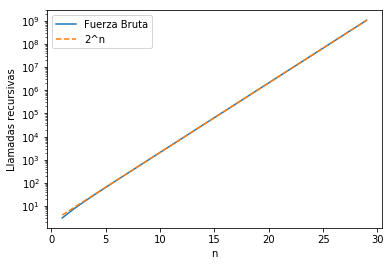
\includegraphics[width=1\textwidth]{img/complejidad/llamadasFB.png} % first figure itself
        \caption{Comparaci\'on de Fuerza Bruta con $2^n$ (Complejidad te\'orica)}
        \label{fig:llamadasFB}
    \end{minipage}\hfill
    \begin{minipage}{0.45\textwidth}
        \centering
        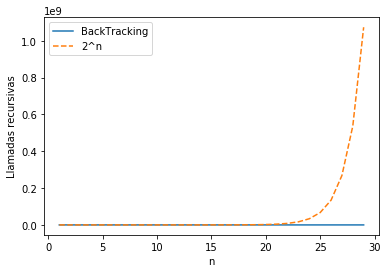
\includegraphics[width=1\textwidth]{img/complejidad/llamadasBack.png} % first figure itself
        \caption{Comparaci\'on de BackTracking con $2^n$ (Complejidad te\'orica)}
        \label{fig:llamadasBack}
    \end{minipage}\hfill
\end{figure}
\begin{figure}[H] 
    \centering
    \begin{minipage}{0.45\textwidth}
        \centering
        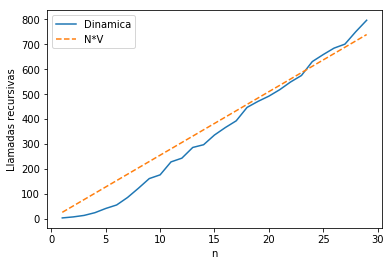
\includegraphics[width=1\textwidth]{img/complejidad/llamadasDin.png} % first figure itself
        \caption{Comparaci\'on de Programaci\'on Din\'amica con $n*V$ (Complejidad te\'orica)}
        \label{fig:llamadasDin}
    \end{minipage}\hfill
\end{figure}

\par Analizando los gr\'aficos podemos ver que en la Figura \ref{fig:llamadasFB} la complejidad del algor\'itmo de Fuerza
Bruta se solapa perfectamente con el de la complejidad te\'orica esperada.
\par Por otro lado, viendo la Figura \ref{fig:llamadasBack} se puede apreciar que la complejidad est\'a muy por debajo
de la complejidad te\'oria gracias a las podas, tal como se esperaba en las hip\'otesis previas a la experimentaci\'on.
\par Por \'ultimo, para el caso de Programaci\'on Din\'amica (Figura \ref{fig:llamadasDin}) se logra ver como la 
complejidad se comporta de manera lineal frente a $V$, aunque se muestra con una pendiente ligeramente
por encima de la complejidad te\'orica esperada. Estimo que se debe a que las soluciones del caso algunos casos bases
se calculan m\'as de una vez a modo de intentar evitar acceder a la posici\'on inv\'alida de la matriz resultados.
N\'otese que hay lugares en los que el gr\'afico se encuenta por debajo de la complejidad te\'orica espeada,
considero que esto se debe al hecho de que no siempre se calculan todas las posibles soluciones de los subproblemas.


\subsubsection{Comparaciones}
\begin{figure}[H] 
    \centering
    \begin{minipage}{0.45\textwidth}
        \centering
        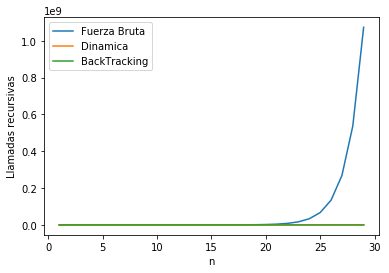
\includegraphics[width=1\textwidth]{img/llamadas/v/todosLlamadasvChico.png} % first figure itself
        \caption{Comparaci\'on de las llamadas recursivas de todos los algor\'itmos con $V = 16$}
        \label{fig:comparaTodosLlamadas}
    \end{minipage}\hfill
    \begin{minipage}{0.45\textwidth}
        \centering
        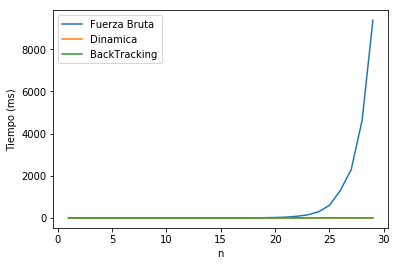
\includegraphics[width=1\textwidth]{img/tiempo/v/todosTiempo.png} % first figure itself
        \caption{Comparaci\'on de los tiempos de ejecuci\'on con $V = 16$}
        \label{fig:comparaTodosTiempo}
    \end{minipage}\hfill
\end{figure}
Tal como se puede ver en las Figuras \ref{fig:comparaTodosLlamadas} y \ref{fig:comparaTodosTiempo} resulta
inviable comparar el algor\'itmo de Fuerza Bruta con los otros dos por motivos de escala, 
raz\'on por la cual de ahora en m\'as solo voy a comparar el de Fuerza Bruta y el de Programaci\'on Din\'amica :
\begin{figure}[H] 
    \centering
    \begin{minipage}{0.45\textwidth}
        \centering
        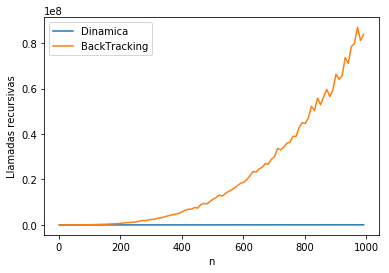
\includegraphics[width=1\textwidth]{img/llamadas/v/llamadasBackDinamicavChico.png} % first figure itself
        \caption{Comparaci\'on de las llamadas recursivas de BackTracking y Programac\'ion Din\'amica con $V = 16$}
        \label{fig:llamadasBackDinamicavChico}
    \end{minipage}\hfill
    \begin{minipage}{0.45\textwidth}
        \centering
        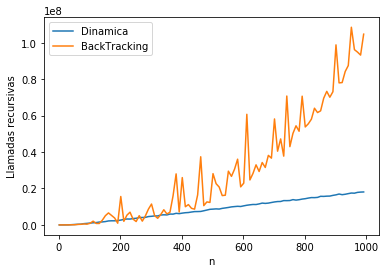
\includegraphics[width=1\textwidth]{img/llamadas/v/llamadasBackDinamicavGrande.png} % first figure itself
        \caption{Comparaci\'on de las llamadas recursivas de BackTracking y Programac\'ion Din\'amica con $V = 6241$}
        \label{fig:llamadasBackDinamicavGrande} 
    \end{minipage}
\end{figure}

\begin{figure}[H] 
    \centering
    \begin{minipage}{0.45\textwidth}
        \centering
        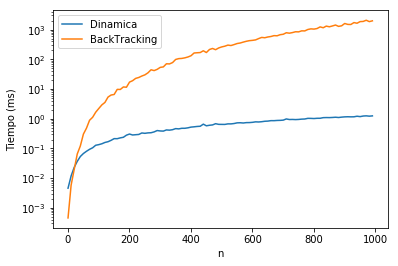
\includegraphics[width=1\textwidth]{img/tiempo/v/tiempoBackDinamicavChico.png} % first figure itself
        \caption{Comparaci\'on del tiempo de ejecuci\'on de BackTracking y Programac\'ion Din\'amica con $V = 16$}
        \label{fig:tiempoBackDinamicavChico} 
    \end{minipage}\hfill
    \begin{minipage}{0.45\textwidth}
        \centering
        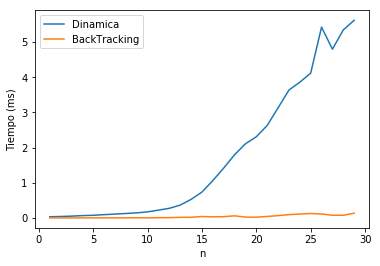
\includegraphics[width=1\textwidth]{img/tiempo/v/tiempoBackDinamicavGrande.png} % first figure itself
        \caption{Comparaci\'on del tiempo de ejecuci\'on de BackTracking y Programac\'ion Din\'amica con $V = 6241$}
        \label{fig:tiempoBackDinamicavGrande} 
    \end{minipage}
\end{figure}

Observando las Figuras \ref{fig:llamadasBackDinamicavChico}, \ref{fig:llamadasBackDinamicavGrande},
\ref{fig:tiempoBackDinamicavChico} y \ref{fig:tiempoBackDinamicavGrande} se logra
ver que los resultados obtenidos se condicen con las hip\'otesis previamente planteadas: con un valor objetivo $V$
``chico'' el algor\'itmo de Programaci\'on Din\'amica realiza menos llamadas (lo cual conlleva a un mayor tiempo
de ejecuci\'on)que el de BackTracking, aunque con un $V$ ``grande'' se da exactamente al rev\'es.
\begin{figure}[H] 
    \centering
    \begin{minipage}{0.45\textwidth}
        \centering
        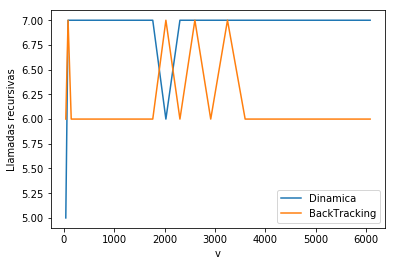
\includegraphics[width=1\textwidth]{img/llamadas/n/backDinNChico.png} % first figure itself
        \caption{Comparaci\'on entre la cantidad de llamadas recursivas entre BackTracking y Programaci\'on
        Din\'amica para $n=2$}
        \label{fig:backDinNChico} 
    \end{minipage}\hfill
    \begin{minipage}{0.45\textwidth}
        \centering
        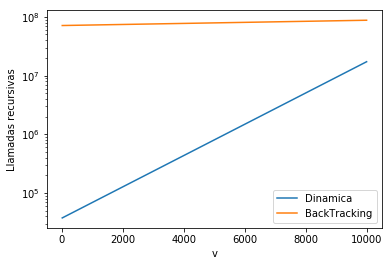
\includegraphics[width=1\textwidth]{img/llamadas/n/backDinNGrande.png} % first figure itself
        \caption{Comparaci\'on entre la cantidad de llamadas recursivas entre BackTracking y Programaci\'on
        \label{fig:backDinNGrande} 
        Din\'amica para $n=29$}
    \end{minipage}
\end{figure}

\par Por \'ultimo, analizando las Figuras \ref{fig:backDinNChico} y \ref{fig:backDinNGrande} podemos notar varias cosas que 
resultan interesantes analizar:
\par Se logra apreciar tanto la independecia de BackTracking respecto a $V$ 
(aunque esperaba que haya alguna dependencia), como la dependencia lineal de Programaci\'on din\'amica con $V$ (teniendo
en cuenta que $n$ se encuentra fijo).
\par Adem\'as, tal como se esperaba, el algor\'itmo de BackTracking se muestra superior en casos de $V$ ``grande'' y 
$n$ ``chico''.
Estimo que esto se debe a que la complejidad depende linealmente de $V$.


\subsection{Experimentaci\'on ``No Llega''}
\subsubsection{Resultads y Comparaciones}

\begin{figure}[H] 
    \centering
    \begin{minipage}{0.45\textwidth}
        \centering
        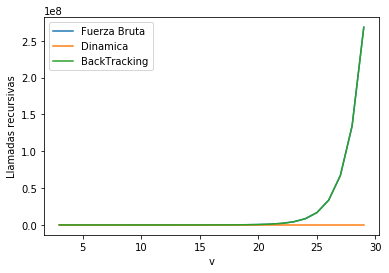
\includegraphics[width=1\textwidth]{img/nollega/todosllamadas.png} % first figure itself
        \caption{Comparaci\'on entre la cantidad de llamadas recursivas entre todos los algor\'itmos}
        \label{fig:todosllamadasnollega} 
    \end{minipage}\hfill
\end{figure}

\begin{figure}[H] 
    \centering
    \begin{minipage}{0.45\textwidth}
        \centering
        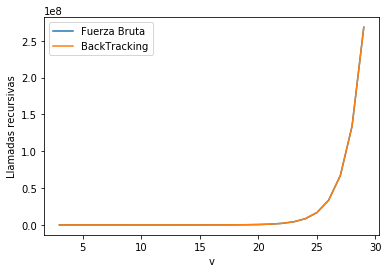
\includegraphics[width=1\textwidth]{img/nollega/backFBllamadas.png} % first figure itself
        \caption{Comparaci\'on entre la cantidad de llamadas recursivas entre los algor\'itmos de
        Fureza Bruta y BackTracking}
        \label{fig:backFBllamadasnollega} 
    \end{minipage}\hfill
    \begin{minipage}{0.45\textwidth}
        \centering
        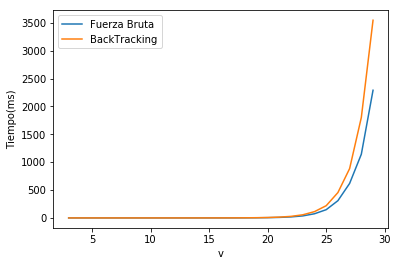
\includegraphics[width=1\textwidth]{img/nollega/backFBtiempo.png} % first figure itself
        \caption{Comparaci\'on entre el tiempo de ejecuci\'on de BackTracking y Fuerza Bruta}
        \label{fig:backFBtiemponollega} 
    \end{minipage}
\end{figure}

\par Tal como se puede ver en las Figuaras \ref{fig:todosllamadasnollega} y \ref{fig:backFBllamadasnollega}
el comportamiento de los algor\'itmos de Fuerza Bruta y BackTracking fue el esperado: realizan la misma cantidad 
de llamadas recursivas ya que en el de BackTracking no se puede realizar ninguna poda. A\'un as\', tal como
lo muestra la figura \ref{fig:backFBtiemponollega} la soluci\'on utilizando BackTracking demora considerablemente
m\'as que el otro. Estimo que esto se debe a las 4 guardas condicionales con las que cuenta (ver Pseudoc\'odigo),
raz\'on por la cual realiza $4$ operaciones extras por vez que se llama a la funci\'on. Esto resulta en $4*2^n$ 
operaciones extras en total.

\begin{figure}[H] 
    \centering
    \begin{minipage}{0.45\textwidth}
        \centering
        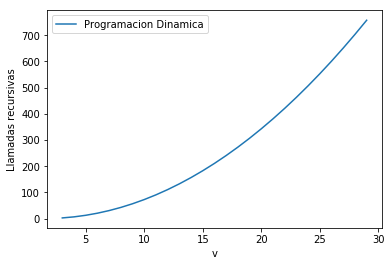
\includegraphics[width=1\textwidth]{img/nollega/dinamicallamadas.png} % first figure itself
        \caption{Cantidad de llamadas recursivas para Programaci\'on Din\'amica}
        \label{fig:dinamicallamadasnollega} 
    \end{minipage}\hfill
    \begin{minipage}{0.45\textwidth}
        \centering
        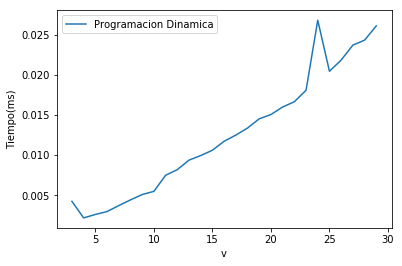
\includegraphics[width=1\textwidth]{img/nollega/dinamicatiempo.png} % first figure itself
        \caption{Comparaci\'on entre el tiempo de ejecuci\'on de BackTracking y Fuerza Bruta}
        \label{fig:dinamicatiemponollega} 
    \end{minipage}
\end{figure}

\par Por \'ultimo, para el caso de la Programaci\'on Din\'amica podemos apreciar un claro comportamiento lineal
respeco a $V$ y $n$ (recordar que $n = V-1$) en las Figuras \ref{fig:dinamicallamadasnollega} y 
\ref{fig:dinamicatiemponollega}. Adem\'as en la Figura \ref{fig:todosllamadasnollega} podemos ver que
el este algor\'itmo realiza muchas menos llamadas recursivas que el resto, validando mis hip\'otesis.
\newpage

\section{Conclusiones}
\par A partir del an\'alisis de los resultados, puedo concluir que no existe un algor\'itmo
que sea siempre mejor que los otros dos ya que dependen de los par\'ametros $n$ y $V$.
Es por esto que a la hora de utilizar la soluci\'on de este problema como subrutina de 
alg\'un otro problema considero de vital importancia analizar las ventajas y deventajas
de cada algor\'itmo seg\'un el \textbf{contexto de uso}.
\subsection{Ventajas}
\subsubsection{Fuerza Bruta}
\begin{itemize}
    \item[\checkmark] Es simple de programar.
    \item[\checkmark] Para un $n$ ``chico'' y un $V$ ``grande'' puede comportarse mejor
    que Programaci\'on Din\'amica.
\end{itemize}

\subsubsection{Backtracking}
\begin{itemize}
    \item[\checkmark] Al realizar podas, no se investiga todo el \'arbol de soluciones
    \item[\checkmark] Para un $n$ y un $v$ tal que $2^n > n*V$ es mejor que el resto.

\end{itemize}

\subsubsection{Programaci\'on Din\'amica}
\begin{itemize}
    \item[\checkmark] Calcula solamente una vez cada subproblema
    \item[\checkmark] Para un $n$ y $n$ tal que $2^n < n*V$ es mejor que los otros dos.

\end{itemize}
\subsection{Desventajas}

\subsubsection{Fuerza Bruta}
\begin{itemize}
    \item[$\times$] Calcula varias veces el mismo subproblema
	\item[$\times$] Siempre recorre todo el \'arbol de soluciones.
	\item[$\times$] Su comlejidad es exactamente $O(2^n)$.
\end{itemize}

\subsubsection{Back Tracking}
\begin{itemize}
    \item[$\times$] En el peor caso (Experimentaci\'on ``No Llega'') realiza la misma.
    cantidad de llamadas recursivas que Fuerza Bruta ya que no puede realizar ninguna poda.
    \item[$\times$] En el peor caso, requiere m\'as tiempo que Fuerza Bruta para
    resolver el problema.
\end{itemize}

\subsubsection{Programaci\'on Din\'amica}
\begin{itemize}
    \item[$\times$] Para un $n$ y $V$ tal que $2^n > n*V$ el algor\'itmo se comporta hasta
    peor que Fuerza Bruta.
    \item[$\times$] Para $n$ y $V$ ``grandes'' es posible que no alcance la memoria disponible
    para almacenar todas las soluciones parciales.
\end{itemize}

\subsection{Conclusion Final}
\par Tal como mencion\'e previamente, la elecci\'on del alg\'oritmo a usar deber\'ia depender
del contexto de uso: si $2^n > n*V$ resulta mejor utilizar Backtracking aunque para $2^n < n*V$
es recomendable utilizar Programaci\'on. No considero que sea aplicable el algor\'itmo de Fuerza
Bruta.

\subsection{Futuros Trabajos}
\par Resultar\'ia interesante hacer un an\'alis sobre cu\'al es el caso promedio para as\'i poder 
determinar cual ser\'ia el algor\'itmo m\'as conveniente de aplicar en un contexto real.
 Adem\'as tambi\'en considero que podr\'ia resultar de inter\'es utilizar un alg\'oritmo 
h\'ibrido entre Backtracking y Programaci\'on Din\'amica: se almacenan las soluciones parciales
pero no se investigan aquellas que por optimalidad o factibilidad no resulten \'util calcular.

\newpage

\section{Ap\'endice}
\begin{figure}[H] 
    \centering
        \centering
        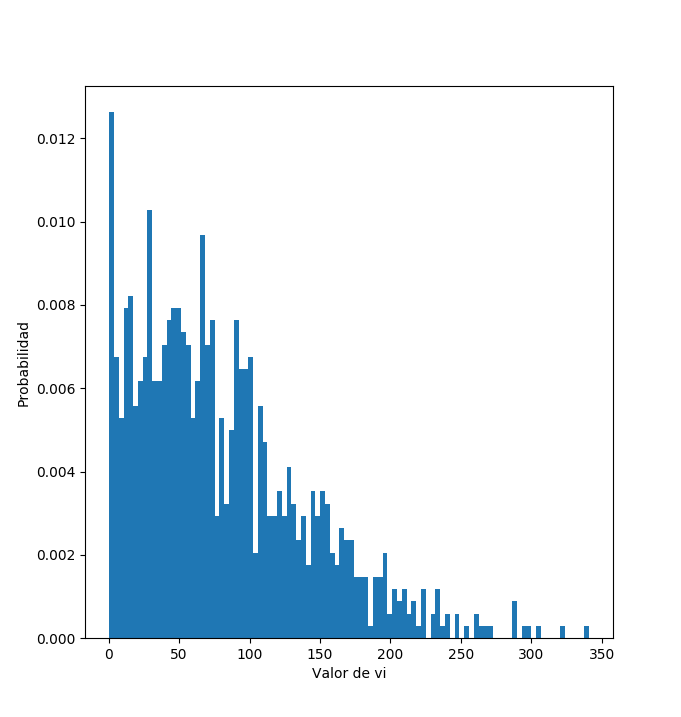
\includegraphics[width=0.7\textwidth]{img/distribucion.png} % first figure itself
        \caption{Ejemplo de la distribuci\'on ``aleatoria'' utlizada en la experimentaci\'on para 
        $n = 1000$ y $vDeseado = 500$}
        \label{fig:tiempoBackDinamicavChico} 
\end{figure}


\end{document}

